\documentclass[tikz,border=2pt]{standalone}
\usepackage{amsmath,amssymb}
\usepackage{tikz}
\usetikzlibrary{arrows.meta,matrix}

\begin{document}
% Jordan normal form: a block-diagonal matrix of Jordan blocks, one chain of generalized
% eigenvectors per block; here blocks of sizes 2, 1 (eigenvalue lambda1) and 2 (lambda2).
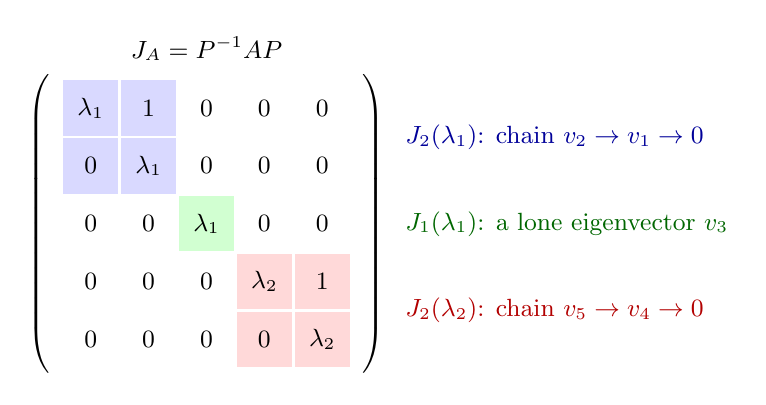
\begin{tikzpicture}[every node/.style={font=\small}]
	\matrix (J) [matrix of math nodes, nodes={minimum size=7mm, anchor=center}, left delimiter=(, right delimiter=), column sep=1pt, row sep=1pt] at (0,0) {
		|[fill=blue!15]| \lambda_1 & |[fill=blue!15]| 1 & 0 & 0 & 0 \\
		|[fill=blue!15]| 0 & |[fill=blue!15]| \lambda_1 & 0 & 0 & 0 \\
		0 & 0 & |[fill=green!18]| \lambda_1 & 0 & 0 \\
		0 & 0 & 0 & |[fill=red!15]| \lambda_2 & |[fill=red!15]| 1 \\
		0 & 0 & 0 & |[fill=red!15]| 0 & |[fill=red!15]| \lambda_2 \\
	};
	\node[anchor=south] at (J.north) {$J_A=P^{-1}AP$};
	\node[blue!60!black, anchor=west] at (2.4,1.1) {$J_2(\lambda_1)$: chain $v_2\to v_1\to0$};
	\node[green!40!black, anchor=west] at (2.4,0.0) {$J_1(\lambda_1)$: a lone eigenvector $v_3$};
	\node[red!70!black, anchor=west] at (2.4,-1.1) {$J_2(\lambda_2)$: chain $v_5\to v_4\to0$};
\end{tikzpicture}
\end{document}
